\documentclass{article}

\usepackage{amsmath, amsthm, amssymb, amsfonts}
\usepackage{thmtools}
\usepackage{graphicx}
\usepackage{setspace}
\usepackage{geometry}
\usepackage{float}
\usepackage{hyperref}
\usepackage[utf8]{inputenc}
\usepackage[russian]{babel}
\usepackage{framed}
\usepackage[dvipsnames]{xcolor}
\usepackage{tcolorbox}

\colorlet{LightGray}{White!90!Periwinkle}
\colorlet{LightOrange}{Orange!15}
\colorlet{LightGreen}{Green!15}

\newcommand{\HRule}[1]{\rule{\linewidth}{#1}}

\declaretheoremstyle[name=Theorem,]{thmsty}
\declaretheorem[style=thmsty,numberwithin=section]{theorem}
\tcolorboxenvironment{theorem}{colback=LightGray}

\declaretheoremstyle[name=Определение,]{prosty}
\declaretheorem[style=prosty,numberlike=theorem]{proposition}
\tcolorboxenvironment{proposition}{colback=LightOrange}

\declaretheoremstyle[name=Principle,]{prcpsty}
\declaretheorem[style=prcpsty,numberlike=theorem]{principle}
\tcolorboxenvironment{principle}{colback=LightGreen}

\setstretch{1.2}
\geometry{
    textheight=9in,
    textwidth=5.5in,
    top=1in,
    headheight=12pt,
    headsep=25pt,
    footskip=30pt
}

% ------------------------------------------------------------------------------

\begin{document}

% ------------------------------------------------------------------------------
% Cover Page and ToC
% ------------------------------------------------------------------------------

\title{ \normalsize \textsc{}
		\\ [2.0cm]
		\HRule{1.5pt} \\
		\LARGE \textbf{{НАИМЕНЬШАЯ ОБЩАЯ НАДСТРОКА}
		\HRule{2.0pt} \\ [0.6cm] \LARGE{Задача о сборке генома} \vspace*{10\baselineskip}}
		}
\date{}
\author{\textbf{} \\ 
		  Валерия 11 З\\
		  ЦПМ\\
		04.10.2023}

\maketitle
\newpage

\tableofcontents
\newpage

% ------------------------------------------------------------------------------

\section{Введение}

\begin{proposition}
    Надстрокой набора строк называется такая строка, что все строки из набора содержатся в ней как подстроки.
\end{proposition}

\begin{proposition}
    Минимальной надстрокой называется надстрока минимальной длины
\end{proposition}

\begin{proposition}
    Строка ${t}$ называется подстрокой строки ${s}$, если существует такой подотрезок ${[l, r]}$ длины ${t}$, такой что ${s_l...s_r = t}$
\end{proposition}

\begin{proposition}
    ${overlap(s, t) - }$ наибольший суффикс строки ${s}$ совпадающий с префиксом ${t.
    }$
    \newline
    Например ${overlap(ABC, BCD) = 2}$
\end{proposition}
% Maybe I need to add one more part: Examples.
% Set style and colour later.


\begin{figure}[htbp]
    \center
    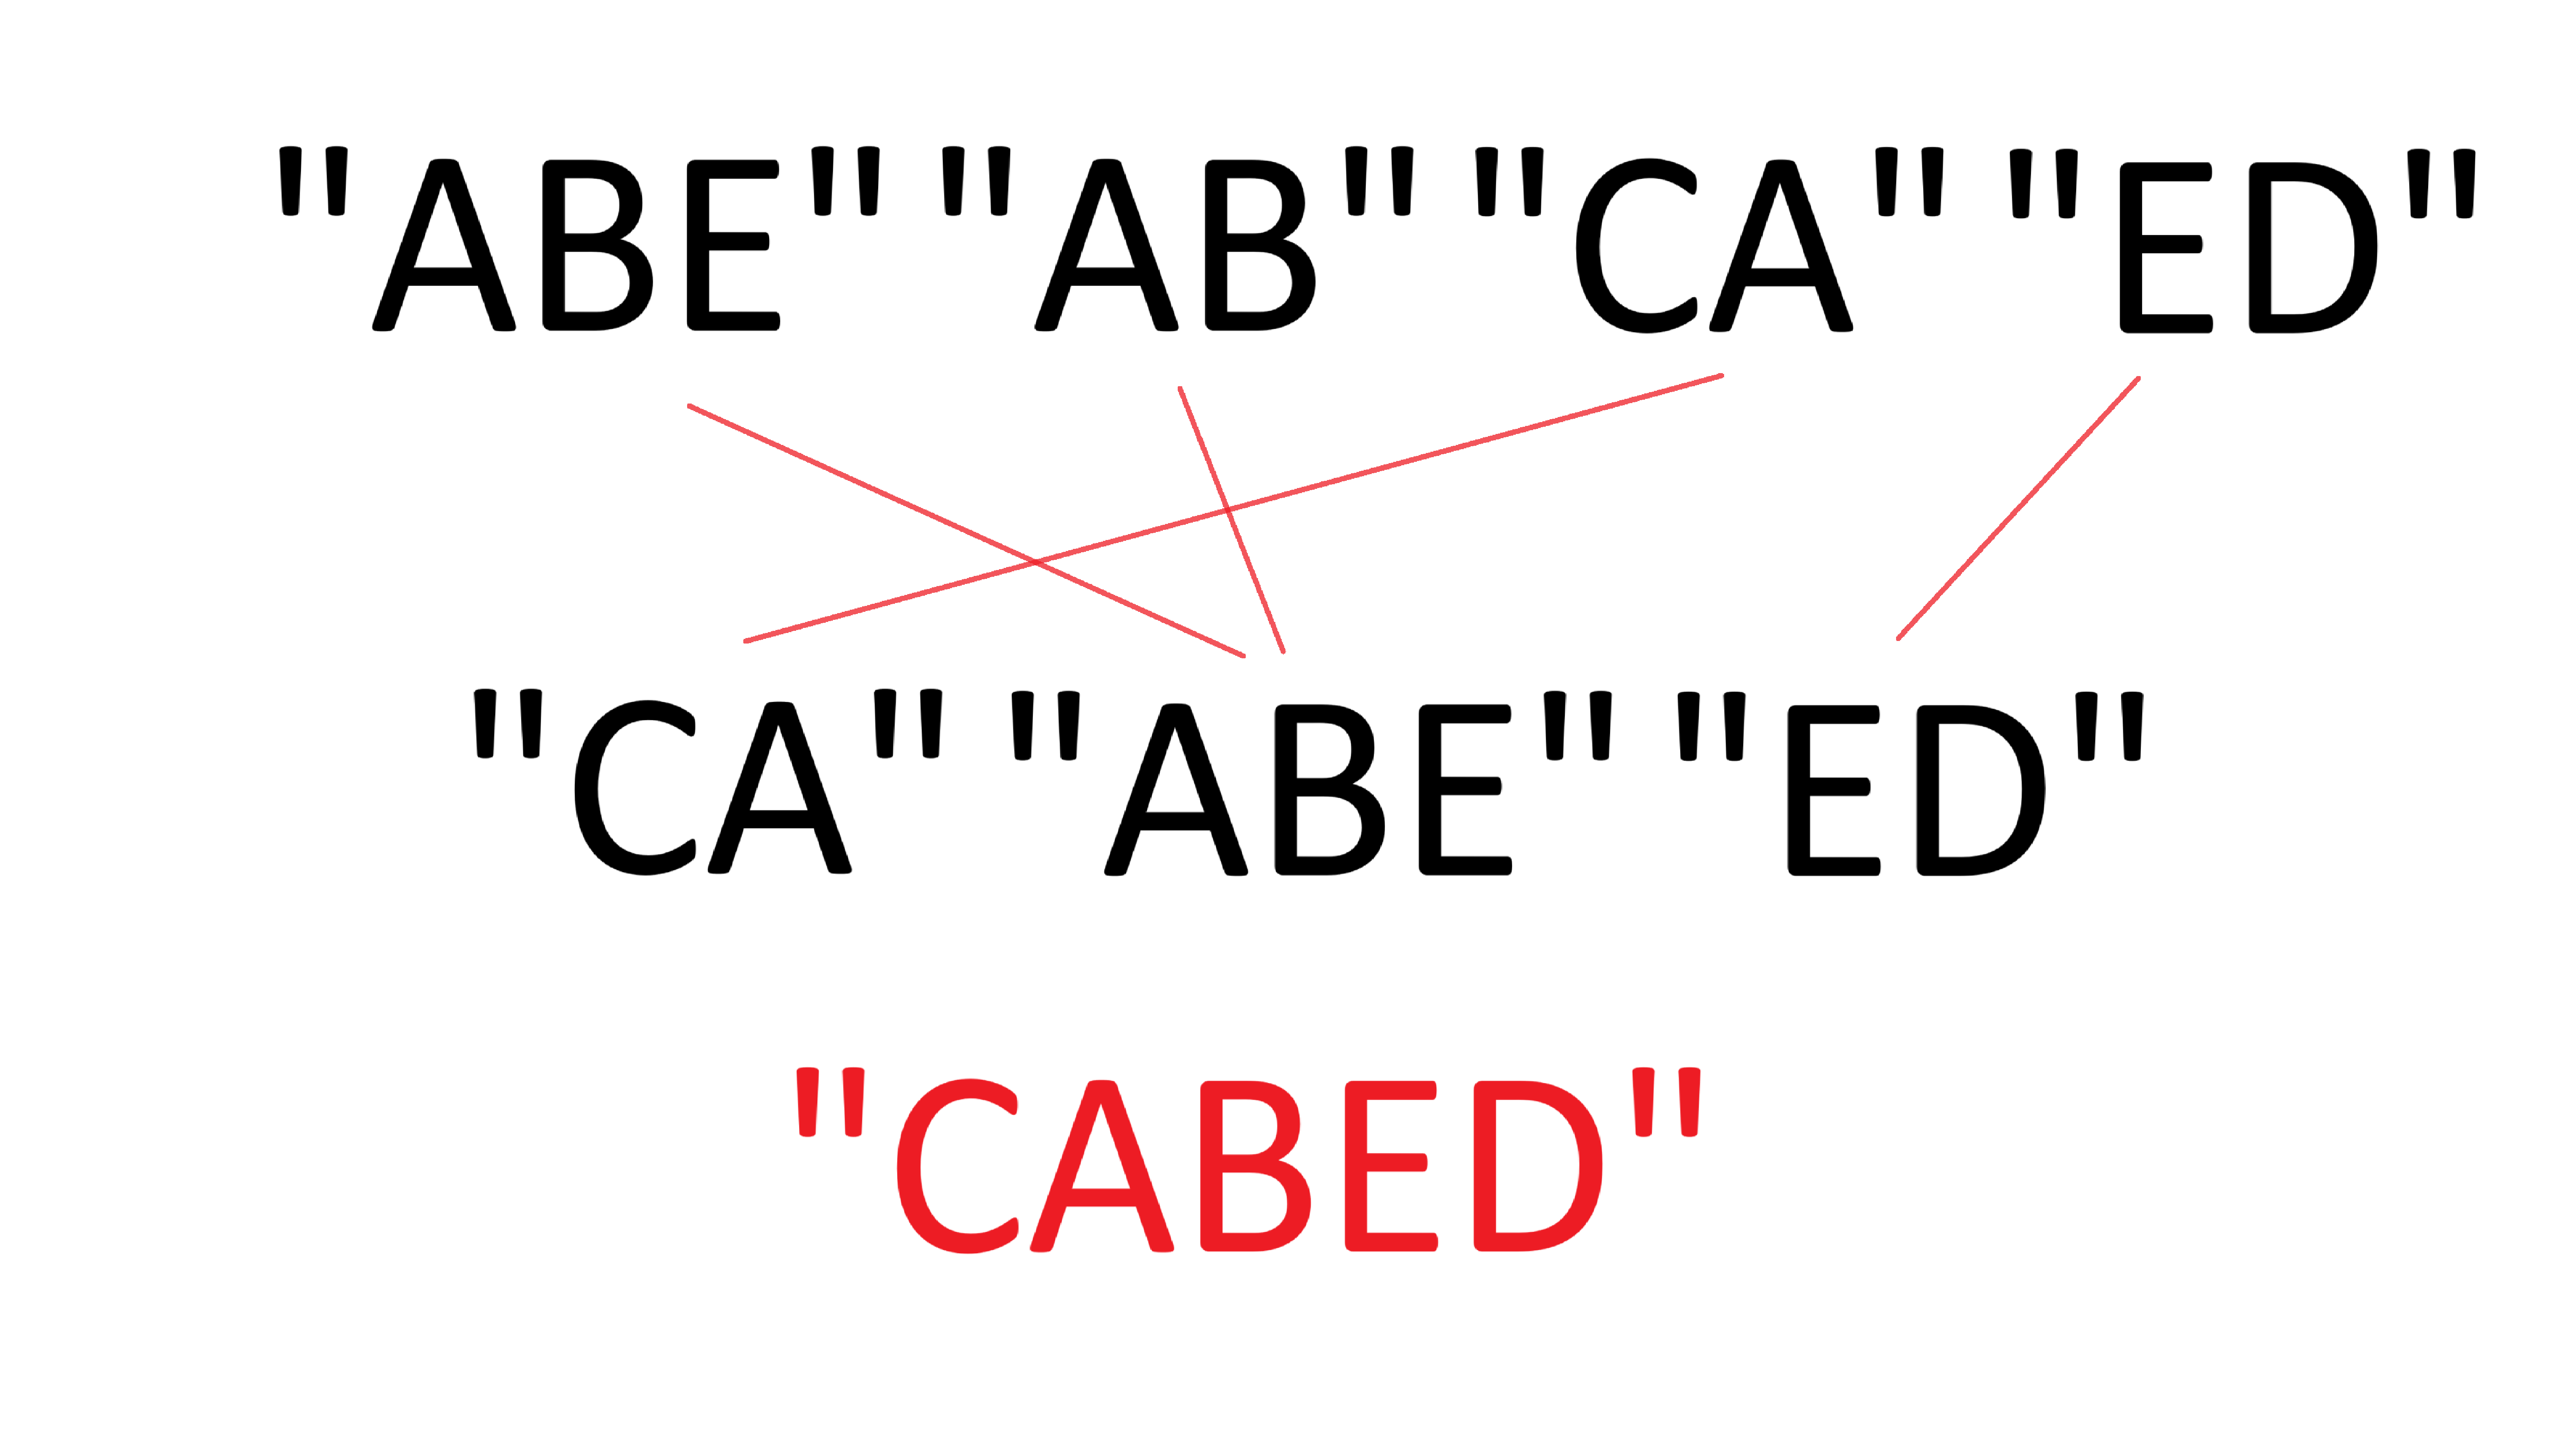
\includegraphics[scale=0.06]{img/example1.png}
    \caption{Пример надстроки}
\end{figure}
\begin{figure}[htbp]
    \center
    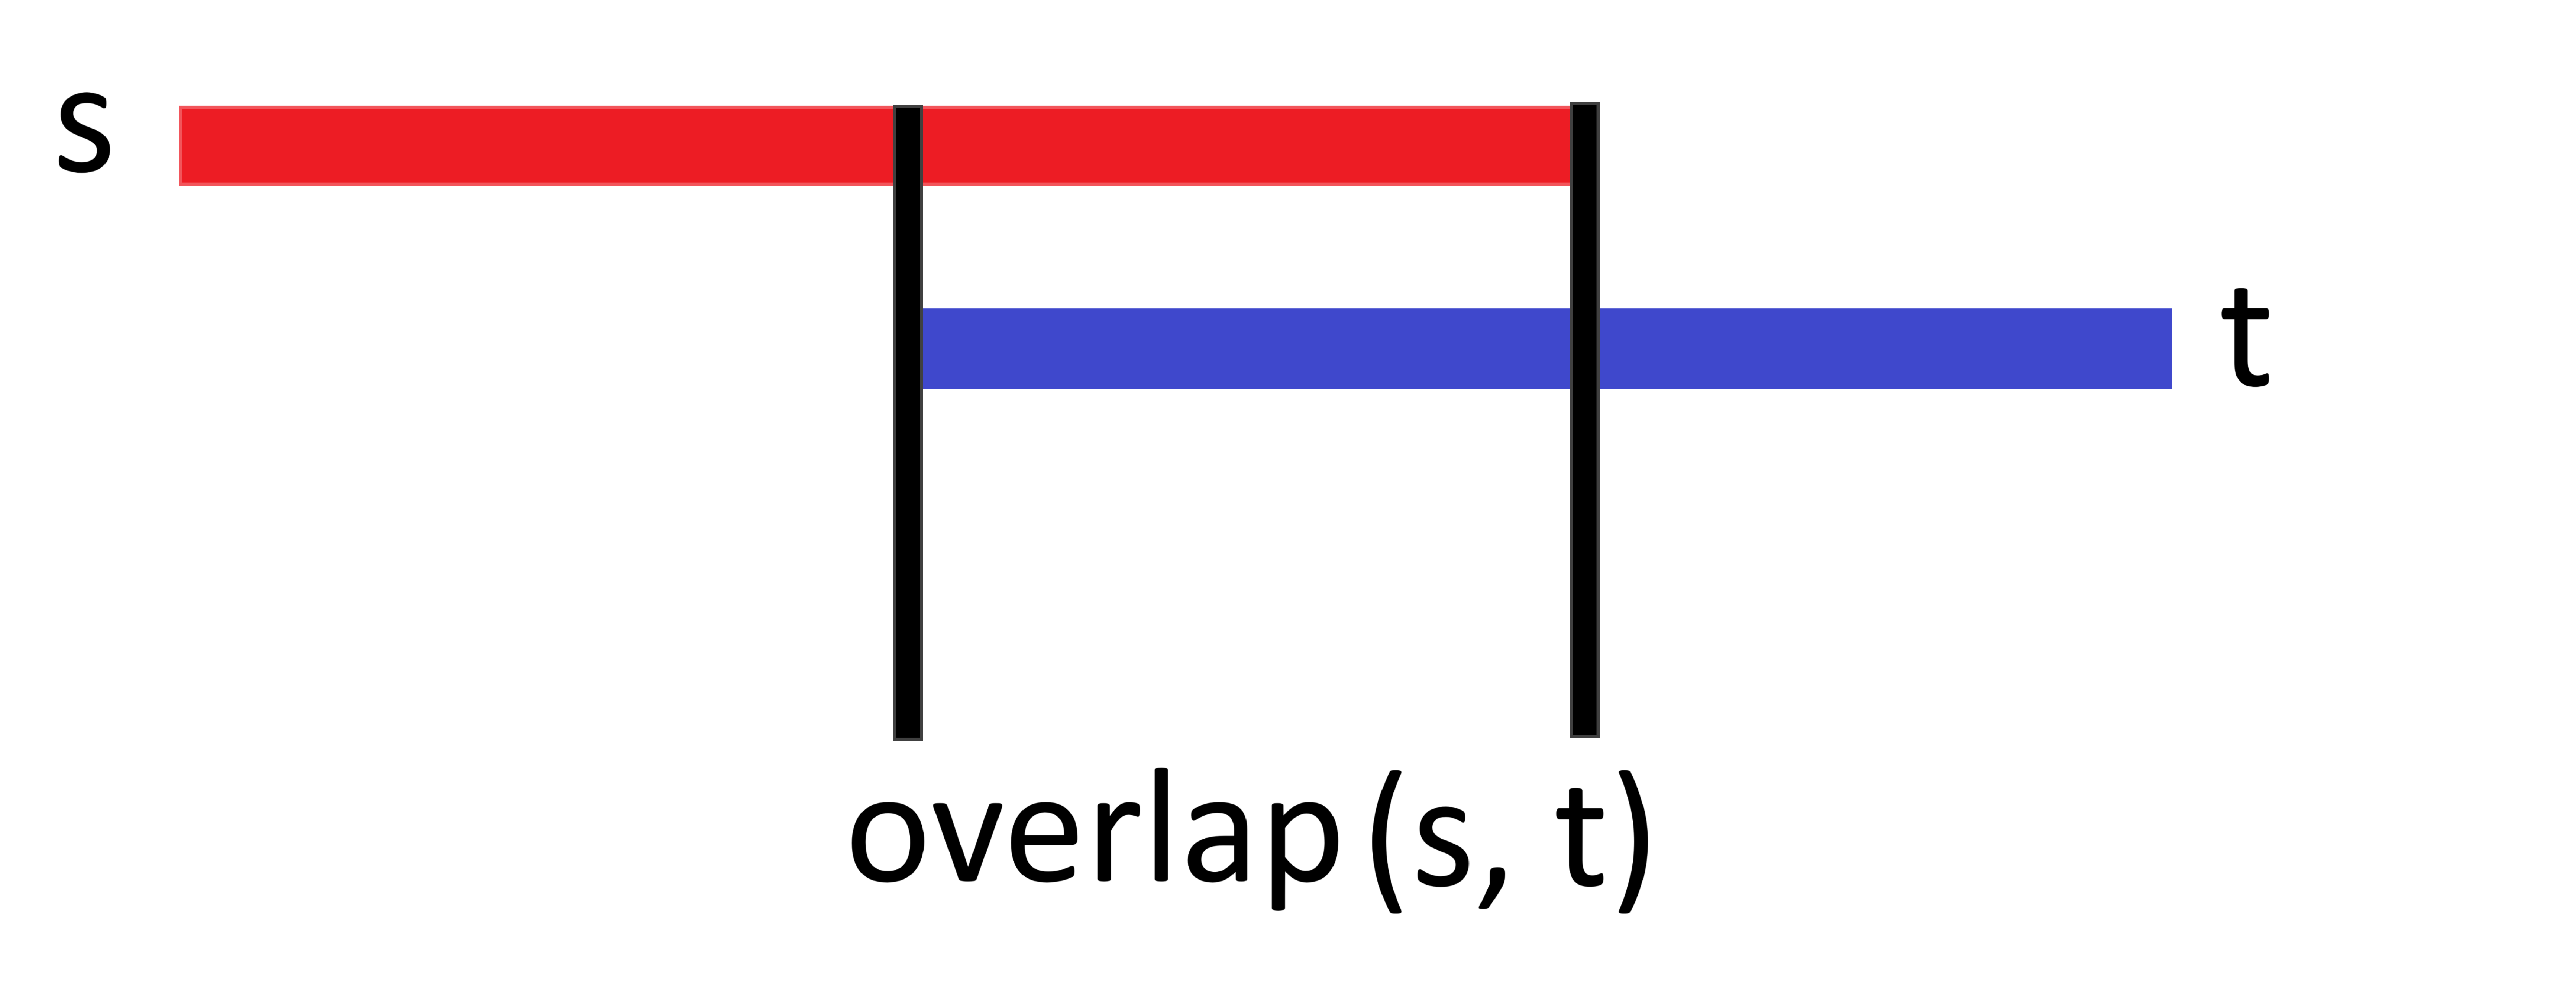
\includegraphics[scale=0.06]{img/example3.png}
    \caption{overlap}
\end{figure}


\newpage
\section{За какое время умеем решать}
\subsection{Перебор всех перестановок}
Заметим, что нам нужно максимимзировать количество ${overlap}$'oв, тогда чтобы гарантированно взять ту, в которой максимальное количество наложений, можно перебрать все перестановки из ${n}$ элементов - строк и каждый раз собирать строку начиная слева направо. \newline
Такое решение будет работать за ${O(n!n)}$, что очень долго даже для $n$ = 20. 

\subsection{Сведение к задачи коммивояжера}
Заметим, что нашу задачу можно представить в виде взвешанного ориентированного графа, где ребро $(u, v)$ будет значить, что у строки ${u}$ есть какой-то {overlap} с ${v}$, а вес на ребре будет обозначать какой именно длины будет этот ${overlap}$. К слову, это будет полный граф, так как у любых двух строк есть ${overlap}$ хотя бы $0$. \newline
После сведения, мы можем решить такую задачу при помощи динамического программирования по подмножествам, перебирая маску вершин, которые мы уже посетили и храня текущую.
\newline
Такое решение будет работать за ${O(2^n n)}$.

\begin{figure}[htbp]
    \center
    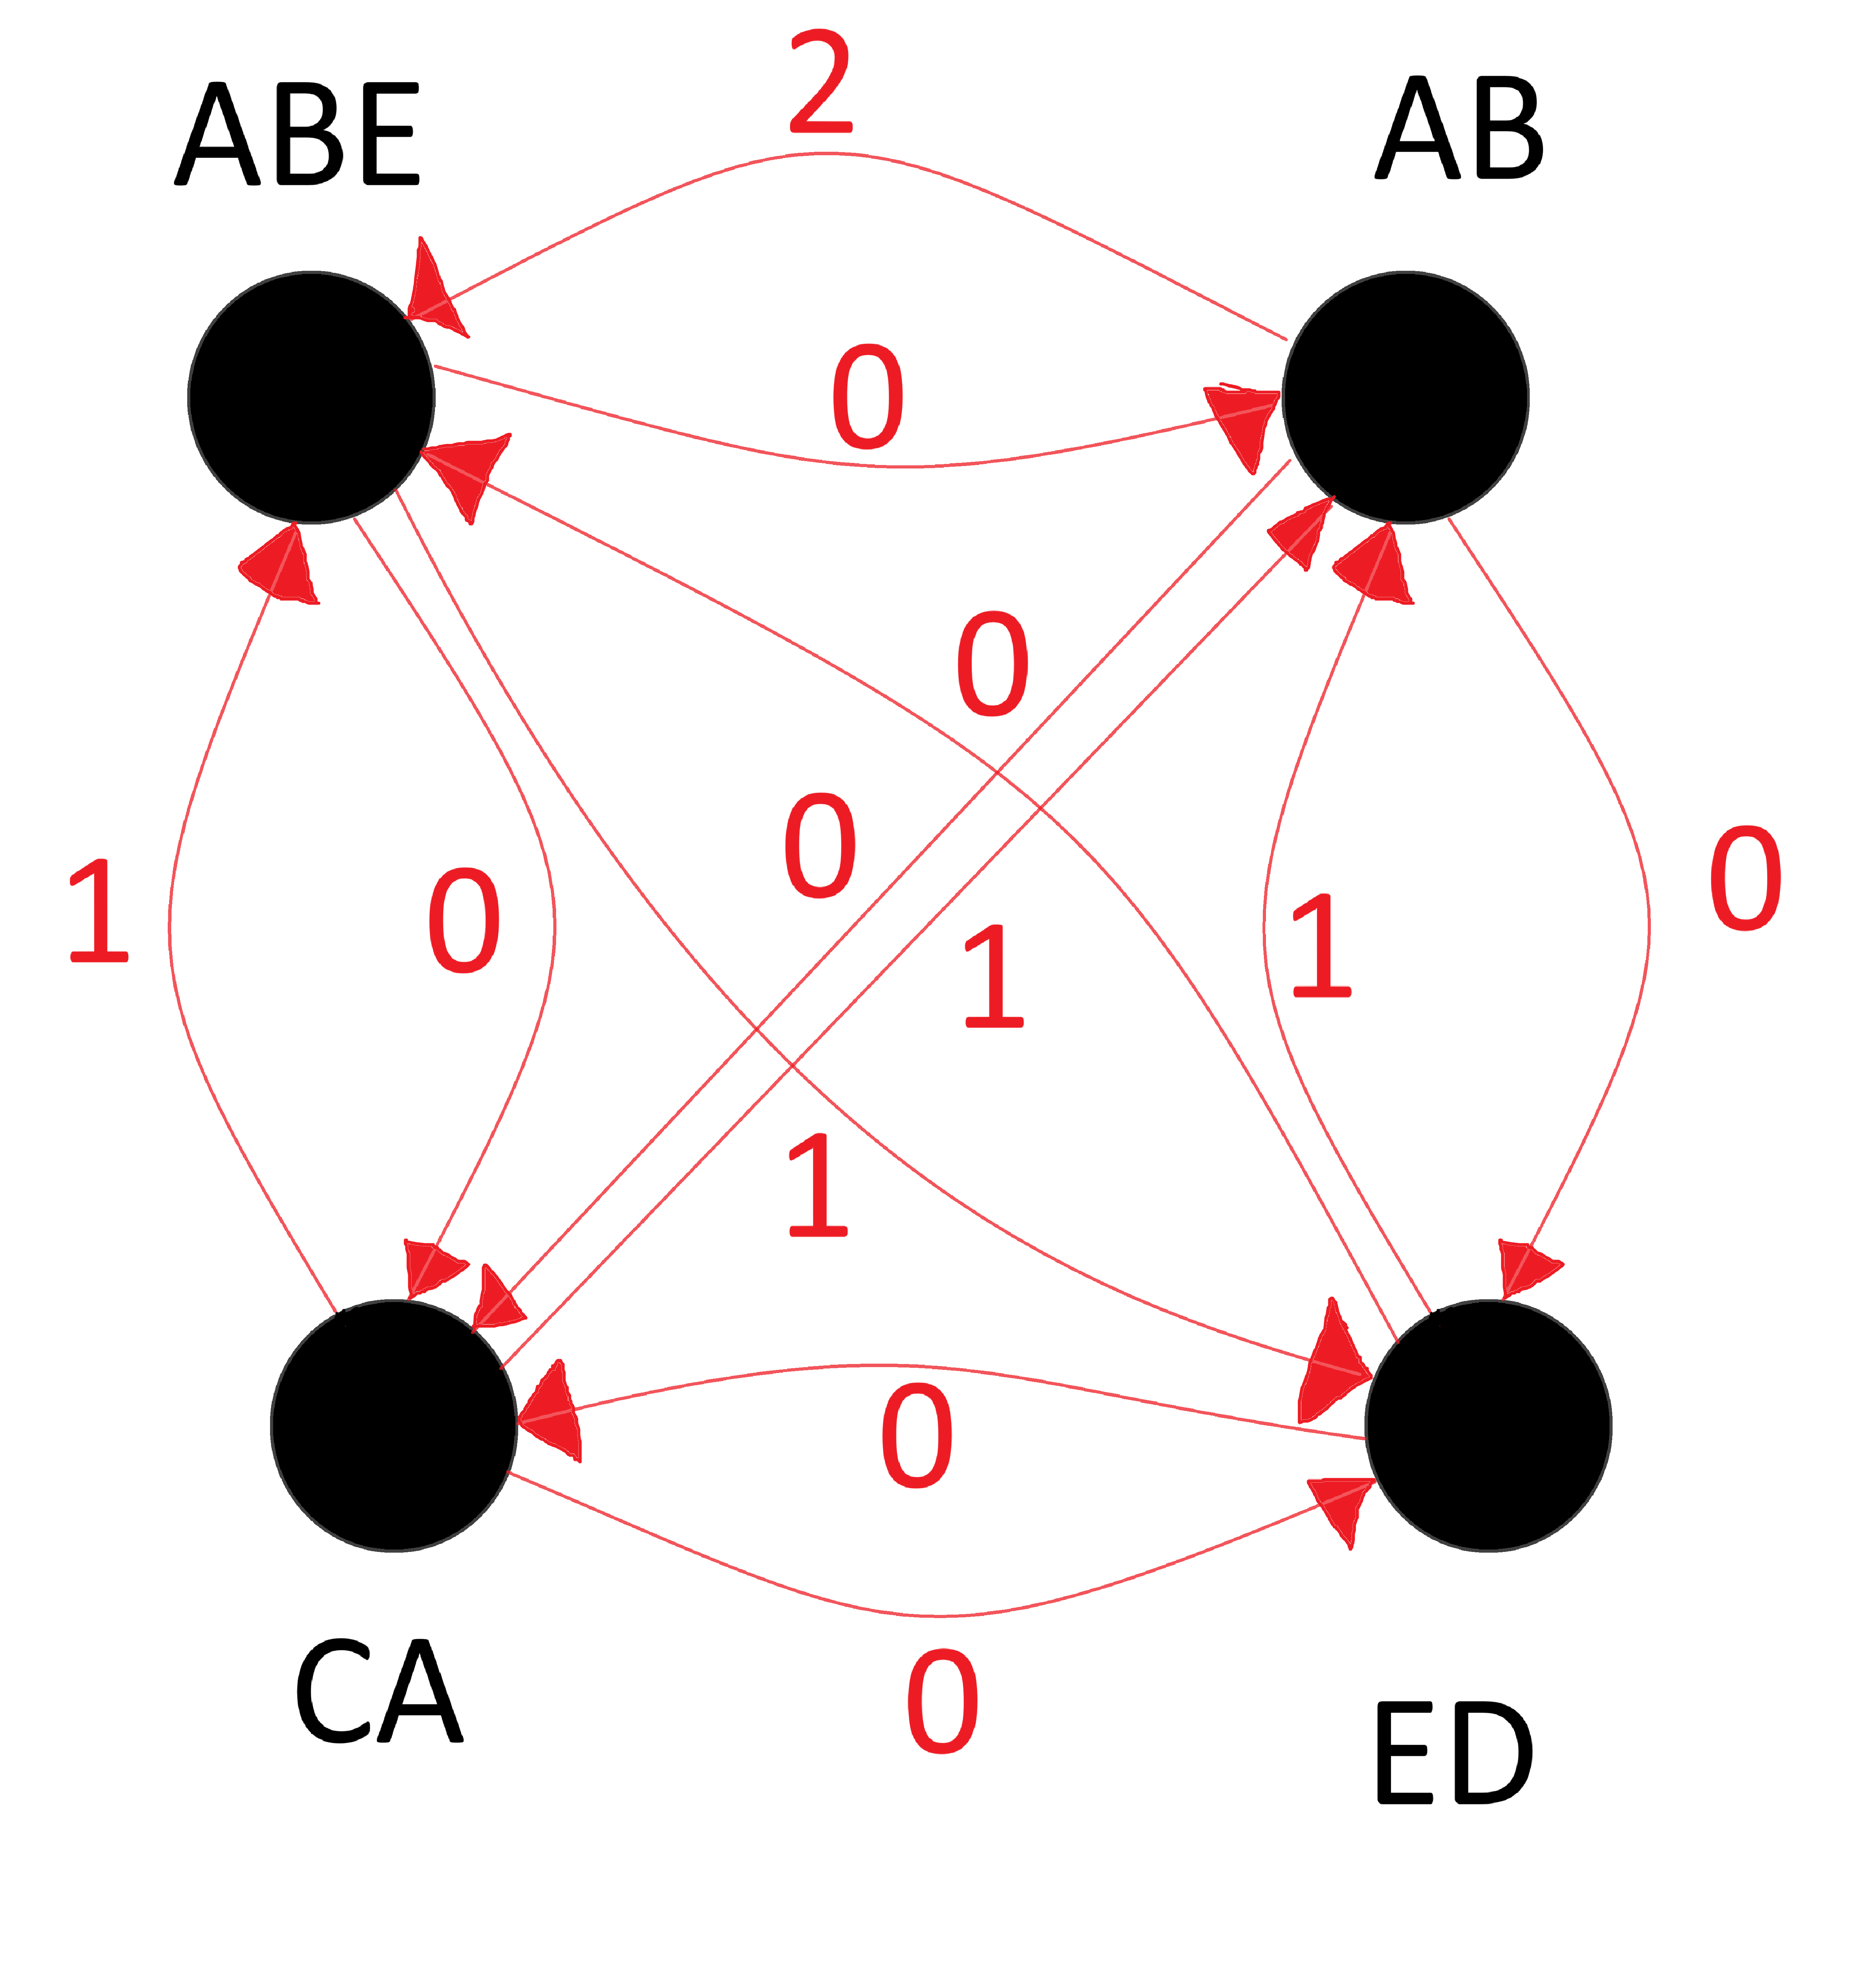
\includegraphics[scale=0.06]{img/example4.png}
    \caption{Представление в виде графа}
\end{figure}
% ------------------------------------------------------------------------------
% Reference and Cited Works
% ------------------------------------------------------------------------------


% ------------------------------------------------------------------------------
\newpage
\section{Жадный алгоритм}
\subsection{Описание алгоритма}
\newline
Я представлю один из самый простых жадных алгоритмов, который можно придумать для этой задачи, его можно улучшать локальными оптимизациями как и в плане асимптотики, так и в плане оптимальности ответа.\newline
Ну хорошо, мы поняли, что нам хочется набрать все самый длинные $overlap$'ы, тогда давайте переберем все пары строк и для каждой насчитаем сначала максимальный суффикс первой строки, совпадающий с перфиксом второй, а потом максимальный префикс первой строки, совпадающий с суффиксом второй. Это можно сделать честно перебрав строки и суффикс, а потом взятием подстроки, этот фрагмент будет работать за $O(n^4)$. Однако это можно улучшить, воспользуемся хешами и тогда то же самое можно будет сделать за $O(n^3)$, подумав еще немного можно заменить цикл, перебирающий префикс на бинарный поиск, так как если существует префикс первой строки длины $k$ совпадающий с суффиксом длины $k$ второй строки, тогда префикс длины $k-1$ тоже будет совпадать с суффиксом длины $k-1$ второй строки, а значит функция монотонна. Тогда асимптотика этого фрагмента будет $O(n^2log(n))$.\newline
Замечательно, теперь мы хотим узнать, какую строку необходимо поставить первой. Давайте для каждой строки насчитаем количество строк, с которыми текущая строка создает $overlap$ величины хотя бы $1$. Теперь пройдемся по всем строкам и из соображения жадности найдем ту, у которой насчитанная выше величина минимальна, обозначим ее $Start$. Далее запустим цикл на $n$ - количество строк и на каждой итерации цикла выберем оптимальную строку для строки $Start$, это будет просто строка, у которой $overlap$ со строкой $Start$ максимальный, назовем выбранную строку за $MaxString$, для того чтобы в дальнейшем случайно не взять эту строку снова, пометим ее
использованной и скажем, что $Start$ теперь равняется $MaxString$ и добавим $MaxString$ в ответ.\newline
Итоговая асимптотика будет $O(Kn^2log(n))$, где $K$ - это то, о чем вы можете узнать в следующем обзадце

\subsection{Как это можно улучшить}
Ну во-первых заметим, что нам не нужны строки, которые являются подстроками других строк, поэтому их можно сразу удалить из массива слов.\newline
Во-вторых, можно поверить в вероятность и выбрать какую-нибудь константу $K$ и $K$ раз случайным образом перемешивать элементы массива и считать для него ответ. Есть вероятность, что таким образом мы улучшим ответ.
В-третьих, вместо того, чтобы просто собирать ответ, можно поддерживать множество строк, которые мы еще не поиспользовали и после нахождения строки, у который $overlap$ со сторокой $Start$ максимальный, объединим их в одну и опять закинем в наше множество (это самая хорошая оптимизация из всех выше перечисленных)
\end{document}
